\cotefile{15}
\scanpage{139}
\margin{138}

\diagram{\begin{tikzcd}
g_{\varphi} \arrow[r,no head] & g \\
g_{\chi} \arrow[u] \arrow[r,no head] & g_{\psi} \arrow[u]
\end{tikzcd}}
\diagram{\begin{tikzcd}
 & G' & \\
V \arrow[r,no head] & G \arrow[u] \arrow[r,"\varepsilon"] & G_m \\
U \arrow[u] \arrow[r] & G^0 \arrow[u] &
\end{tikzcd}}

Soit $k'$ une extension algébrique de $k$, d'où un foncteur
$\mathcal M\longrightarrow\mathcal M'$ catégorie de motifs sur $k'$ engendrée
par les $M\otimes_k k'$, $M\in\mathcal M$.
\[
\mathcal M^{(0)}\longrightarrow\mathcal M'^{(0)}
\]
d'où
\[
g'\longrightarrow g
\]
\diagram{\begin{tikzcd}
G' \arrow[r,hook] \arrow[d] & G \arrow[d] \\
\Gamma' \arrow[r,hook,no head] \arrow[d,equal] & \Gamma \arrow[d,equal] \\
G'/G'^0 & G/G^0
\end{tikzcd}}
L'hom $G'\hookrightarrow G$ \deleted{définit} est un mono et
définit un isom sur les comp. connexes

\diagram{\begin{tikzcd}
g'_{\varphi'} \arrow[r,no head] & g' \\
g'_{\chi'} \arrow[u] \arrow[r,no head] & g'_{\psi'} \arrow[u]
\end{tikzcd}\quad\longrightarrow\quad\begin{tikzcd}
g_{\varphi} \arrow[r,no head] & g \\
g_{\chi} \arrow[u] \arrow[r,no head] & g_{\psi} \arrow[u]
\end{tikzcd}}

En particulier, on trouve
\[
g'_{\chi}\;-\;g_{\chi}\qquad
 g'_{\psi'}\longrightarrow g_{\psi}
\]
\[
U'\xrightarrow{\sim}U\qquad G'^0\simeq G^0.
\]

\diagram{\begin{tikzcd}
\deleted{\unsure{V'}} \arrow[r] & G' \\
U' \arrow[u] \arrow[r] & G'^0 \arrow[u]
\end{tikzcd}\quad\longrightarrow\quad\begin{tikzcd}
V \arrow[r,no head] & G \\
U \arrow[u] \arrow[r,no head] & G^0 \arrow[u]
\end{tikzcd}}

\scanpage{141}
$K$ extension finie de $\mathbb Q$
\[
T_K=\prod_{K/\mathbb Q}G_m,\qquad
N_{K/\mathbb Q}:T_K\longrightarrow T_{\mathbb Q}=G_m,\qquad
\deleted{\unsure{V_K}}\quad V_K(\subset T_K)=\operatorname{Ker}N_{K/\mathbb Q};
\]
\[
1\longrightarrow V_K\longrightarrow T_K\longrightarrow G_m\longrightarrow1
\]
\margin{\textcircled{\S\,1}}
\uline{NB} Si $E_K$ unités, alors $E_K\cap V_K(\mathbb Q)$ est d'indice $1$ ou $2$
dans $E_K$, et contient $E_{1K}$ [unités complètes y compris à l'$\infty$]

\uline{Proposition} Soit $V'_{\deleted{\unsure{K}}}$ \inserted{$=V_K/R$} un groupe quotient de $V_K$.
Les conditions suivantes sont équivalentes

(i) L'image de $E_1$ dans $V'_{\deleted{\unsure{K}}}(\mathbb Q)$ est finie, i.e.
$R\cap E$ est d'indice fini dans $E$.

(ii) Il existe un ``module'' $m$ de $K$ tel que
$T_{\deleted{\unsure{K}}}\longrightarrow T_m=T/\overline E_m$
est nul sur $R$, i.e. $T'=T/R_{\deleted{\unsure{E}}}$ est majoré par le quotient $T_m$ de $T$.

(iii) $(V')_{\mathbb R}$ est un tore compact.

(iv) Si $L$ \deleted{\unsure{L}} est le plus-grand sous-corps Weilien de $K$, et
$L_0=L\cap\mathbb R\subset L$ (d'indice $1$ ou $2$ dans $L$)
\deleted{le plus-grand sous-corps tot réel de $K$,}
\deleted{Alors l'hom $i_{K,L}:T_{\deleted{\unsure{K}}L_0}\longrightarrow T_K$
(qui applique $V_K$ dans $V_L$) applique,}
$R$ \deleted{est donc} \inserted{contient} le noyau de l'\deleted{épi}morphisme
\[
\deleted{\unsure{T}}\quad
V_K\xrightarrow{N_{K/L}}V_L\xrightarrow{\mathrm{can}}V_L/\operatorname{Im}V_{L_0}.
\]
où $V_{L_0}\longrightarrow V_L$ est induit par l'inclusion
$T_{L_0}\hookrightarrow T_L$; i.e.
$V'_K$ ``est'' un quotient de $V_L/\operatorname{Im}V_{L_0}$.

\uline{Dém} (i) signifie qu'il existe $F\deleted{E}\subset E_1$
\inserted{ss-gr.} d'indice fini dans $E_1$ telle que $V'$ soit majoré par
$\deleted{T}\inserted{V}/\overline F$ ($\overline F$, adhérence zariskienne de $F$)
i.e. $T'$ majoré par $V/\overline F$; comme les $E_m$ sont d'indice fini
dans $E_1$, on voit que $(\mathrm{ii})\longrightarrow(\mathrm{i})$, et
$(\mathrm{i})\Rightarrow(\mathrm{ii})$ car tout sous-groupe d'indice fini de $E_1$
\deleted{contient} (ou de $E$, c'est kif) contient un $E_m$ (Chevalley).

$(\mathrm{i})\Longrightarrow(\mathrm{iii})$ Car soit \deleted{$E$}
$F=R\cap E$, de sorte que $V'$ est majoré par $V/\overline F$,
\deleted{si} donc $V'_{\mathbb R}$ majoré par $V_{\mathbb R}/\overline F$
(où maintenant $\overline F$ désigne l'adhérence zariskienne dans $V_{\mathbb R}$),
\inserted{et $V'(\mathbb R)=V_{\mathbb R}(\mathbb R)/\overline F(\mathbb R)$.}
Or on sait que
\[
V(\mathbb R)\subset
(\mathbb R^{*r_1}\times\mathbb C^{*r_2})
\inserted{\simeq\mathbb R_+^{*(r_1+r_2)}\times(\mathbb Z/2\mathbb Z)^{r_1}\times U^{r_2}}
\]
[le \deleted{\unsure{diviseur}} sous groupe des syst. $(\lambda_i)(\mu_j)$
tels que $\prod\lambda_i\prod|\mu_j|^2=1$
\inserted{i.e. $(\rho_i)(\varepsilon_j),(u_h)$ tel que $\prod\rho_i=1$}],
et $E_1$ (donc $F$) en est un
\margin{140}

\scanpage{142}
Pour expliciter la condition (iii), il reste donc : expliciter les tores
quotients \inserted{\uline{compacts}} de \deleted{$\unsure{T_L}$} $V_L$, et
prouver que ce sont les quotients de $V_L/V_{L_0}$.

\deleted{$V_{L_0}$ n'a manifestement pas de \inserted{tore} quotient compact
\inserted{sauf le gr. unité}, donc le plus grand quotient compact de $V_L$
est majoré par $V_L/V_{L_0}$.}

\par\noindent
\deleted{\mbox{\begin{minipage}[c]{\linewidth}
\deleted{Pour voir} Il reste : prouver que ce dernier est compact.
C'est trivial si $L=L_0$. Sinon, (faisant $L=K$ pour simplifier les notations),
considérons \deleted{i.e. que $V_L/V_{L_0}$} \inserted{la première partie}
i.e. : prouver \unsure{que}
\[L_{\mathbb R}\simeq\mathbb R^{\unsure{r_1}}\qquad L_{0\mathbb R}=\]
\end{minipage}}}
\par

\uline{Corollaire 1} Supposons $K$ wailien, soit $K_0=K\cap\mathbb R$,
\deleted{et} Alors $V_K/V_{K_0}$ est compact, et $V_{K_0}$ n'a d'autre
\inserted{tore} quotient compact que le gr unité.
\deleted{L'image de $E_K$ dans}
De plus $E_K\cap V_{K_0}(\mathbb Q)$ est d'indice fini dans $E_K$;
\inserted{i.e. l'image de $E_{1K}$ dans $V_K/V_{K_0}$ est finie.}

Il suffit \inserted{(pour la 1ère assertion)} de prouver l'énoncé analogue
après extension de la base $\mathbb Q-\mathbb R$.
Alors $K_{0\mathbb R}\simeq\mathbb R^r$, \deleted{\unsure{et est un}}
\inserted{donc $T_{L_0}$ et à fortiori}
$V_{L_0}$ est un \inserted{tore} splitté, donc tout quotient est splitté;
donc compact seulement s'il est \deleted{\unsure{le}} nul.
D'autre part $V_K/V_{K_0}$ est compact: c'est trivial si $K=K_0$,
sinon on aura $K_{\mathbb R}\simeq\mathbb C^{*r}$, et
\[
V_K/V_{K_0}\simeq T_K/T_{K_0}\simeq
\deleted{\prod_{\unsure{r}}}
\bigl[(\prod_{\mathbb C/\mathbb R}G_m)/G_m\bigr]^r\simeq U^r
\]
est compact.

La dernière \unsure{insertion|assertion} signifie \deleted{\illegible{1} \unsure{signifie}} que $E_{K_0}$ est d'indice
fini dans $E_K$. Or les rangs sont respectivmt, si $[K_0:K]=r$,
$r-1$ et $r-1$, O.K.

$(\mathrm{iv})\Longrightarrow(\mathrm{i})$ Résulte immédiatement du fait que
$N_{L/K}$ applique $E_{1K}$ dans $E_{1L}$, et de la dernière
assertion du corollaire.
\margin{141}

\scanpage{143}
\unsure{ss-gpe|ss-gr.} \uline{discret} de rang $r_1+r_2-1$, de sorte que le quotient
$V(\mathbb R)/F$ est compact. Il en est à fortiori de même de
$V(\mathbb R)/\overline F$, donc de $V'_{\mathbb R}$ qu'il majore.

\deleted{$(\mathrm{iii})\Longrightarrow(\mathrm{i})$, car si $V'_{\mathbb R}$ est compact,
i.e. $V'(\mathbb R)$ compact, considérant $V'(\mathbb R)$ comme quotient de
$\mathbb R_+^{*(r_1+r_2-1)}\times(\mathbb Z/2\mathbb Z)^{r_1}\times U^{r_2}$,
on voit que ce sera un quotient de de $(\mathbb Z/2\mathbb Z)^{r_1}\times U^{r_2}$,
or l'image de $E_1$ dans ce dernier est déjà finie [l'image}

$(\mathrm{iii})\Longrightarrow(\mathrm{iv})$ Si $V'_K$ est un tore compact, le groupe
des car. à \deleted{coeff} valeurs dans \deleted{$\unsure{\widetilde K}$}
$\overline{\mathbb Q}\subset\mathbb C$, regardé comme module sous
$G=\operatorname{Gal}(\widetilde K/K)$
($\widetilde K\deleted{\subset\mathbb Q}$ une ext. de $K$ finie galoisienne sur $\mathbb Q$)
est telle que $\tau\in G$ (la conjugaison complexe) y opère par $-\operatorname{id}_M$,
\inserted{donc est central, donc $M$ est un $G'=G/P$-module, où $G'$}
\deleted{Donc si $G'=G/H$ est le quotient de $G$ qui opère fidèlement sur $M$,}
est le grpe de Galois de la plus gde ss-ext. Weilienne
\deleted{\unsure{a défini} une extension $K'\subset\widetilde K$}
$K'$ de $\widetilde K$.
\inserted{Prouvons d'abord que $R\supset\operatorname{Ker}(N_{K/L}|V_K)$
i.e. que $V'$ est un \uline{quotient} de $V_L$ considéré comme quotient de $V_K$.}
\deleted{Alors $\unsure{K'}$ \unsure{est} $\tau'=\operatorname{Im}(\tau\mapsto G')$
est dans le centre de $G'$, donc $K'$ est Weilienne.}

\margin{\diagram{\begin{tikzcd}
\deleted{\widetilde K} \arrow[d] & \\
K \arrow[r,no head,"Q"] \arrow[d,no head,"H"'] & \widetilde K \arrow[d,no head,"P"] \arrow[ddl,no head,bend left=35,"G"] \\
L=K\cap K' \arrow[r,no head] \arrow[d,no head] & K' \arrow[dl,no head,"G'=G/P"] \\
\mathbb Q &
\end{tikzcd}}}

$I_K$ \inserted{$=G/Q$} espace homogène sous $G$ des hom de $K$ dans $\overline{\mathbb Q}$

$\mathbb Z[I_K]$ [groupe libre engendré par $I$] groupe des caractères de $T_K$
à valeurs dans $\overline{\mathbb Q}$, comme $G$-module.

\deleted{$\unsure{N|M}\subset\mathbb Z[I]$ tel que}

$\mathbb Z\subset\mathbb Z[I_K]$ fonctions constantes sur $I$

\diagram{\begin{tikzcd}
\mathbb Z \arrow[r,phantom,"\subset" description] & N \arrow[dr,phantom,"\subset"{description,sloped}] \arrow[r,phantom,"\subset" description] & \mathbb Z[I_K] \\
\mathbb Z \arrow[u,dotted,"\wr"] \arrow[rr,phantom,"\subset" description] & & \mathbb Z(I_L) \arrow[u,hook]
\end{tikzcd}}

$N$ sous $G$-module, tel que $\tau$ opère sur $N/\mathbb Z$ par $-\mathrm{id}$,
donc $P$ y opère trivialmt; donc $H$ opère trivialmt sur $N$, donc
$N\subset\mathbb Z[I_K]^P=\mathbb Z[P\backslash I_K]$
\deleted{$\subset\mathbb Z$}.
Or $P\backslash I_K=I_L$, donc on trouve \deleted{$\subset$}
$N\subset\mathbb Z[I_L]$, ce qui signifie que le quotient $V'$ de $V_K$ est majoré par $V_L$.

\margin{$I_K=G/Q$\par
$I_L=G/PQ=P\backslash I_K\deleted{Q}$\par
$\tau\in G$\par d'ordre $2$}
\margin{142}

\scanpage{144}
\uline{Corollaire 2} Parmi les $V'$ satisfaisant les conditions de la proposition,
il y en a un maximal \deleted{$\unsure{E}\;V_{\mathrm{cpt}}$}
\inserted{$V_K^{\mathrm{cpt}}$}, correspondant à un $R$ minimal.
Le $R$ correspondant est connexe. Avec les notations de (iv),
\inserted{$N_{L/K}$ induit un isom
$V_K^{\mathrm{cpt}}\simeq V_L/V_{L_0}=V_L^{\mathrm{cpt}}$; le $R$ correspondant}
est aussi le produit $[\operatorname{Ker}(N_{K/L})].V_{L_0}$,
\deleted{et l'hom}

Seule la dernière assertion demande encore une vérification.
Comme $N_{K/L}(\lambda)=\lambda^r$ si $\lambda\in L$, on voit que le $R$ cherché
contient $V_{L_0}$, et aussi bien sûr $\operatorname{Ker}(N_{K/L})$.
\deleted{Ou bien} donc $R$ contient le produit $R'$.
\deleted{Alors} Comme $\lambda\mapsto\lambda^r$ de $V_{L_0}$ dans lui-même est un épimorphisme,
on voit que $N_{L/K}$ induit un isom.
\[
V_K/(\operatorname{Ker}(N_{K/L}).V_{L_0})\simeq
V_L/N_{L/K}(V_{L_0})\simeq V_L/V_{L_0},
\]
ce qui établit le Corollaire 2.

On désigne par $S_K^0$ le quotient $T_K/R$, donc on a une suite exacte
\margin{\deleted{\unsure{$(*)$}}}
\[
1\longrightarrow V'_K\longrightarrow S_K^0\xrightarrow{\varepsilon}G_m\longrightarrow1
\]
s'insérant dans une suite exacte
\diagram{$(*)\quad$\begin{tikzcd}
1 \arrow[r,no head] & V_K \arrow[r,no head] \arrow[d,"\mathrm{can}"'] & T_K \arrow[r,no head,"N_K"] \arrow[d,"\mathrm{can}"] & G_m \arrow[r,no head] \arrow[d,equal] & 1 \\
1 \arrow[r,no head] & V'_K \arrow[r,no head] & S_K^0 \arrow[r,no head] & G_m \arrow[r,no head] & 1
\end{tikzcd}}

Pour $K$ variable, $S_K^0$ est contravariant en $K$ pour $N_{K'/K}$,
ainsi que le diagramme $(*)$ [\deleted{les tores} la fonction du plus gd
quotient cpct est fonctoriel en le tore $T$ sur $\mathbb Q$].
Il est aussi covariant \deleted{\unsure{-}} par $i_{K,K'}$ [$=$ raison]
mais bien sûr cette injection n'est plus compatible avec $\varepsilon$,
ou. de façon précise, pour $K\subset K'$
\margin{143}

\scanpage{147}
\margin{\uline{parler de sous-schémas $\Sigma$ de $E\otimes K$.}}
\margin{\textcircled{\S\,2}}
Soient $E,K$ deux extensions de $\mathbb Q$, \deleted{$\Sigma$}
$\mathfrak U$ un idéal de \inserted{$E_K=$} $E\otimes_{\mathbb Q}K$,
$\overline K$ une clôture algébrique de $K$.
On dit que $\mathfrak U$ définit une CM-structure sur $E$, relativement à $K$,
si l'idéal $\mathfrak U'$ de
$E\otimes_{\mathbb Q}\unsure{\overline K^{\sharp}|\overline K}=E_K\otimes_K\overline K$
\uline{engendré} par $\mathfrak U$ correspond à un sous-ensemble \inserted{$\Sigma$}
de l'ensemble \deleted{$\unsure{I}$} \deleted{$I_E$}
$\operatorname{Spec}E_{\unsure{\overline K^{\sharp}|\overline K}}
\simeq\operatorname{Hom}_{\mathrm{alg}}(E,\overline K)$ qui est tel que pour tout
élément $\tau$ de $G=\operatorname{Gal}(\overline K/K)$ qui est une conjugaison,
on ait $\tau(\Sigma)=(\operatorname{Spec}E_{\overline K})-\Sigma$.
Noter que ceci implique que pour $g\in G$, on a aussi
$g\tau g^{-1}(\Sigma)=(\operatorname{Spec}E_{\overline K})-\Sigma=\tau\Sigma$,
donc $\tau^{-1}g\tau g^{-1}(\Sigma)=\Sigma$, donc $\Sigma$ est invariant
\deleted{dans} \inserted{par} le ss-groupe \deleted{\unsure{de}} fermé invariant $H$
engendré par les $\tau^{-1}g\tau g^{-1}$.
Cela signifie que, si $K_0\subset K$ est le corps de définition de l'idéal
$\mathfrak U$ de $E_K$, le corps $K_0$ \inserted{$=k_{\Sigma}$} est \uline{weilien};
\deleted{et} il est d'ailleurs weilien \uline{non réel}, car $\tau(\Sigma)\ne\Sigma$
[puisque sinon on aurait $\operatorname{Spec}E_{\overline K}=\varnothing$, ce qui n'est pas].

\deleted{Supposons maintenant également $K$ fini sur $\mathbb Q$.}
\inserted{Soit $\overline{\mathbb Q}$ une clôture \uline{algébrique} de $\mathbb Q$}
\deleted{Alors} de groupe de Galois $G$.
Alors $E,K$ correspondent à des espaces homogènes compacts sous $G$, soient $I_E,I_K$.
La donnée de $\mathfrak U$ correspond à celle d'une partie fermée de $I_E\times I_K$,
invariante par $G$. Choisissons un plongt $K\subset\overline{\mathbb Q}$,
donc $I_K\simeq G/Q$, $Q$ le sous-groupe de $G$ qui laisse fixe les éléments de $K$.

\deleted{L'hypothèse} \deleted{Remplaçant} \inserted{Prenant} $K$ pour \inserted{$\overline{\mathbb Q}=$}$\overline K$ a pour effet de remplacer
$I_K$ par son pt origine $y$ \deleted{et} (plongt de $K$ dans $\overline{\mathbb Q}$),
et $\Sigma$ devient $\Sigma_y=\Sigma\cap(I_E\times y)$.
\inserted{Soit $\Sigma'=(I_E\times I_K)-\Sigma$, d'où $\Sigma'_y$.}
L'hypothèse est que pour tte conj. complexe $\tau\in G$,
\[
\deleted{(\tau\times1)(\Sigma\cap(I_E\times y))=(I_E-\Sigma}
\qquad
(\tau\times1)\Sigma_y=\deleted{I_E-}\Sigma'_y
\]
\[
\deleted{(\tau\times1)\Sigma'_y=I_E-\Sigma'_y}
\]
i.e.
\par\noindent
\deleted{\mbox{\begin{minipage}[c]{\linewidth}
\unsure{que pour|que peut} écrire aussi
\[
\left\{\begin{array}{l}
(\tau\times1)\Sigma_y\subset I_E-\Sigma\\
(\tau\times1)\Sigma'_y\subset I_E-\unsure{\Sigma'_y|\Sigma_y}
\end{array}\right.
\]
\end{minipage}}}
\par
\margin{146}

\scanpage{148}
Il est évident que la condition envisagée ne dépend pas du choix de l'immersion
$K\hookrightarrow\overline{\mathbb Q}$, \deleted{\unsure{donc}} i.e. du choix de $y$,
et peut donc s'écrire
\[
(*)\qquad(\tau\times1)\Sigma=\Sigma'\qquad\text{pour tte conjugaison }\tau
\]
\[\deleted{(\tau\times1)\Sigma\subset}\]
Je dis qu'elle équivaut aussi à
\[
(**)\qquad(1\times\tau)\Sigma\subset\Sigma'\qquad\text{pour tte conjugaison }\tau
\]
En effet, comme $(\tau\times\tau)\Sigma=\Sigma$, la relation $(*)$ équivaut à
$(\tau\times1)(\tau\times\tau)\Sigma=\Sigma'$ i.e. $(1\times\tau)\Sigma=\Sigma'$.

\uline{Donc la condition envisagée est symétrique en} $E,K$.

\par\noindent
\deleted{\mbox{\begin{minipage}[c]{\linewidth}
Considérons maintenant le sous-corps $K_0$ de $K$, corps de définition de
$\Sigma_y$: c'est \inserted{le corps des invariants du sous-groupe $H\subset G$,}
\unsure{par} des $g\in G$ tels que
\[
\deleted{g\Sigma_y\subset\Sigma_y}\qquad
(g\times1)\Sigma_y=\Sigma'_y,
\]
ce qui \deleted{implique} \inserted{équivaut}
\deleted{pour tte conjugaison} (comme $K_0$ donc $H$ doit être indépendant du choix de $y$) à
\[
\deleted{(g\times1)(\unsure{g^{-1}|g}\times g^{-1})\Sigma_y=\Sigma_y}\qquad
(g\times1)\Sigma\subset\unsure{\Sigma'|\Sigma}.
\]
\deleted{\unsure{par ci-dessus}\quad $\unsure{gK}$}
[vérification: $\Sigma_{y'}=(h\times h)\Sigma_y$ pour $h$ tel que $hy=y'$, donc
\[
(g\times1)\Sigma_{y'}=(g\times1)(h\times h)\Sigma_y=
\deleted{(g\times1)\Sigma_y}
(1\times h)(gh\times1)\Sigma_y=(1\times h)\Sigma'_y=\Sigma'_{y'},
\]
et comme $\Sigma=(g^{-1}\times g^{-1})\Sigma$, cela équivaut :
$(g\times1)(g^{-1}\times g^{-1})\Sigma=\Sigma'$,
i.e. à $(1\times g^{-1})\Sigma=\Sigma$, ou encore $(1\times g)\Sigma=\Sigma$]. Donc
\end{minipage}}}
\par

\uline{NB} Soit $\mathfrak U$ une structure CM sur le couple $E,K$,
et considérons $E\hookrightarrow E'$, $K\hookrightarrow K'$ des extensions de corps.
Alors l'idéal $\mathfrak U'=\mathfrak U(E'\otimes K')$ de $E'\otimes K'$ est une structure
\inserted{CM} de Sh. Tan. sur $E',K'$, et \uline{réciproquement}.
\deleted{La théorie de Galois}

\deleted{On dit que} Soit $\mathfrak U$
\deleted{structure CM sur $E,K$} \inserted{un idéal de $E\otimes K$}, envisagé
comme idéal de $E_K$; $\mathfrak U$ a un ``corps de définition'' $K_0\subset K$.
Je dis que celui-ci est invariant par extension du corps $E\longrightarrow E'$
(vérification triviale). De ceci
\margin{147}

\scanpage{149}
résulte que l'on a un plus petit couple $(E_0,K_0)$ $(E_0\subset E,\ K_0\subset K)$
tel que $\mathfrak U$ provienne d'un idéal de $E_0\otimes K_0$.
On a vu que $E_0,K_0$ sont weiliens non réels. Si $E_0$ est fini sur $\mathbb Q$,
de degré $2d$, alors $K_0$ est fini sur $\mathbb Q$, de degré $\leq\binom{2d}{d}$
[car le ss-groupe des $g\in G$ qui invarient une partie à $d$ éléments
dans un ens. à $2d$ éléments est d'indice $\leq\binom{2d}{d}$].
\deleted{Si $K$ f $K$} Si $E$ fini sur $\mathbb Q$ de degré $2d$, alors
$\mathfrak A(\Sigma):=(E\otimes K)/\mathfrak U$ est fini sur $K$ de degré $d$,
et réciproqt.

Soient $E,K$ deux extensions de $\mathbb Q$, $t$ un bimodule sur $E,K$, i.e. un module
sur $E\otimes K$. On dit que $t$ est du type CM si $t$ est monogène, et son annulateur
est un $\mathfrak U$ de type CM. Les bimodules de type CM \inserted{sur $E,K$} sont
classifiés, à isom près, par les structures CM $\deleted{\mathfrak U}\Sigma$ sur le couple $E,K$.

Un tel $t$ définit \inserted{(si \deleted{E} $K$ fini sur $\mathbb Q$, i.e. $t$ fini sur $E$),}
un hom
\[
\psi_\Sigma:T_K\longrightarrow T_E
\]
dont l'action, sur les pts rationnels sur $\mathbb Q$ (pour fixer les idées) est donnée par
\[
\psi_\Sigma(x)=\operatorname{dét}_{t/E}(x_t)\,;
\]
Ou si on préfère, en termes de la fonction caractéristique de $\Sigma$
(qui est ouvert et fermé), notée \deleted{aussi $\Sigma$} $1_\Sigma$
\[
\psi_\Sigma(x)=N_{E\otimes K/E}(x1_\Sigma^{\deleted{\Sigma}})
\]
Si $K'$ est une extension finie de $K$, \inserted{et $E'$ ext. de $E$,}
donnant lieu à un $\Sigma'$ dans $E'\otimes K'$, on aura commutativité dans
\diagram{\begin{tikzcd}[column sep=large]
T_{K'} \arrow[r,"N_{K'/K}"] \arrow[rrr,bend right=24,"\psi_{\Sigma'}"'] &
T_K \arrow[r,no head,"\psi_\Sigma"] & T_E \arrow[r,no head,"i_{E'/E}"] & T_{E'}
\end{tikzcd}}
\margin{148}

\scanpage{150}
Ceci montre que l'on est réduit : étudier \inserted{$\psi_\Sigma$ dans} le cas où
$K=K_0$, $E=E_0$ (donc $E,K$ weiliens et finis).

Identifiant les duaux de $T_E,T_K$ à valeurs dans $\overline{\mathbb Q}$ à
$\mathbb Z^{I_E}$, $\mathbb Z^{I_K}$, on constate que l'hom
\inserted{(comp.ble : $G$)} sur les \deleted{\unsure{caract.}} groupes de caractères
défini par $T_E$:
\diagram{\begin{tikzcd}\mathbb Z^{I_E}\arrow[r,no head]&\mathbb Z^{I_K}\end{tikzcd}}
est donné par la matrice $1_\Sigma$ considéré comme une fonction
\deleted{caractéristique} sur $I_E\times I_K$).
\uline{Donc la connaissance de} $\Sigma$ \uline{équivaut à celle de} $\psi_\Sigma$
(cette dernière n'étant d'ailleurs pas quelconque\ldots).

Choisissons une clôture algébrique $\overline E$ de $E$,
\deleted{supposons $K$} \inserted{supposons $K$ fini (degré $2d'$) sur $\mathbb Q$,}
alors la structure $\Sigma$ équivaut à la donnée d'un ensemble \deleted{de} d'hom
\[
\sigma_1,\ldots\sigma_{d'}:K\longrightarrow\overline E
\]
\deleted{conjugués} tels que pour tte conj. $\tau$ de $G=\operatorname{Gal}(\overline E|\mathbb Q)$,
les $\{\tau\sigma_i,\sigma_i\}$ font l'ens de \uline{tous} les hom $K\longrightarrow\overline E$.
On aura alors
\[
\psi_\Sigma(x)=\sigma_1(x)\sigma_2(x)\cdots\sigma_{d'}(x)
\]
Si $K$ est weilien,
\deleted{donc si $x\in K_r$ (ss-corps tot. réel),}
\inserted{les $\sigma_i|K_r$ font \deleted{un ens} l'ens des hom
$K_r-\overline E$, et on trouve}
\deleted{on aura $\tau\sigma_i(x)=\sigma_i(x)$, donc}
\[
\deleted{\psi_\Sigma(x)^2=N_K}
\]
\[
\psi_\Sigma|T_{K_r}=N_{K_r/\mathbb Q}
\]
Par suite, $\psi_\Sigma$ s'annule sur $V_{K_r}\subset T_{K_r}\subset T_K$.
De ceci, et du §1, on conclut que \uline{si} $K$ \uline{fini sur} $\mathbb Q$,
alors $\psi_\Sigma:T_K\longrightarrow T_E$ \uline{se factorise par} $S_K^0\longrightarrow T_E$:
\margin{149}

\scanpage{151}
\diagram{\begin{tikzcd}[column sep=large]
T_K\arrow[r,"\mathrm{can}"]&S_K^0\arrow[r,"\psi_\Sigma"]&T_E
\end{tikzcd}}
\margin{par abus de notation}
Rappelons-nous de l'homomorphisme
\[
i_K:G_{m\mathbb Q}\longrightarrow S_K^0
\]
je dis qu'on a
\[
\alpha)\qquad\boxed{\psi_\Sigma i_K=i_{E/\mathbb Q}}
\]
Comme on a
\[
i_K^{\deleted{d}}(x)^{d'}=i_{K/\mathbb Q}(x)\qquad(x\in\mathbb Q^*)
\]
la relation $\alpha$ équivaut (en élevant : puissance $d'$ième) à
\[
\deleted{i_K}\,\psi_\Sigma(x)=x^{d'}\qquad\text{pour }x\in\mathbb Q^*
\]
qui est trivialt vérifiée.

[\unsure{\textcircled{b}} Quelle est l'image de $\psi_\Sigma$? Il revient au $=$ de
donner l'image de $V'_K$, le ss-groupe compact maximal de $S_K^0$, car
\[
\psi_\Sigma(S_K^0)=\psi_\Sigma(V'_K).i_{E/\mathbb Q}(G_m)
\]
On va bien sûr se \deleted{ramener} \inserted{borner} au cas
$E=E_0$ \ldots.]

\uline{Question} Pour $K$ fixé, \inserted{tel que $S_K^0\xrightarrow{\unsure{\varepsilon_K}}G_m$
ne soit pas un isom,} les hom $\psi_\Sigma:S_K^0-T_E$ associés aux diverses
structures CM \uline{sur $K$} \deleted{sont} forment-ils une \uline{famille fidèle}?
\inserted{On peut supposer $K$ weilien non réel.}
Soit $\Sigma:\{\sigma_1\ldots\sigma_{d'}\}$ une structure CM sur $(K,\overline{\mathbb Q})$.
\deleted{Alors si $x\in K^*$ est} \inserted{Soit, pour $\forall\,1\leq i\leq d'$,}
$\Sigma_i$ \deleted{tel que} la structure CM déduite de $\Sigma$ en remplaçant
$\sigma_i$ par $\overline\sigma_i=\tau\sigma_i$. Alors, si $x\in K^*$ est tel que
$\psi_\Sigma(x)=1$ et $\psi_{\Sigma_i}(x)=1$, on aura par quotient que
$\sigma_i(x)=\overline\sigma_i(x)$, donc si ceci est vrai pour $\forall x$,
on aura $x\in K_r$. De plus, \deleted{On} $\psi_\Sigma(x)=1$ revient alors à
$N_{K_r/\mathbb Q}(x)=1$, donc $x=V'_{K_r}$.
Donc l'image de $x$ dans $S_K^0$ est $1$.
Cet argument vaut aussi en remplaçant $\mathbb Q$ par une alg. quelconque sur $\mathbb Q$
\deleted{[car $\bigcap\operatorname{Ker}(\sigma_i,\overline\sigma_i)=K_r$ est
stable par}
\margin{150}

\scanpage{152}
(NB $K_r=\bigcap_i\operatorname{Ker}(\sigma_i,\overline\sigma_i:
K\rightrightarrows\overline{\mathbb Q})$ est stable par tt changement de base
$\mathbb Q\longrightarrow\Lambda$). Donc
\[
\operatorname{Ker}\psi_\Sigma\cap\bigcap_{1\leq i\leq d'}\operatorname{Ker}\psi_{\Sigma_i}
=1\qquad\text{dans }S_K^0
\]

\uline{Question} Regardons les hom. $\psi_\Sigma:S_K^0\longrightarrow T_E$, avec $E$
\uline{quadratique}. Y en a-t-il assez, du moins en filtrant sur $K$ croissants?
Or un $E$ a, relativt à une \deleted{\unsure{E}} extension $K$ de $\mathbb Q$,
\deleted{deux} $0$ structure CM si $E$ ne pas plonger dans $K$, et deux exactement
dans le cas contraire \inserted{(correspond. aux plongts)}
\inserted{[L'hom $\psi_K$ correspondant est \deleted{\operatorname{Tr}_{K/E}} $N_{K/E}$.}
Donc pour $K$ fixé, les hom $\psi_\Sigma:S_K^0-T_E$ correspondent par paires conjuguées
aux plongts $E\longrightarrow K$; donc pour voir s'il y en a assez, il faut voir s'il y a
``assez'' de sous-corps quadratiques de $K$.
Si $K$ \inserted{(supposé Weilien)} n'est pas \inserted{(dés. $L$ ce ss-corps)}
engendré par ses sous-corps quadratiques, i.e. si \deleted{le groupe de} \inserted{$K$ n'est}
pas galoisien de groupe de Galois $(\mathbb Z/2\mathbb Z)^N$, alors le noyau de
$N_{K/L}:S_K^0-S_L^0$ est un tore de dim $>0$ qui est dans le noyau de tous les
$\psi_K$ envisagés.
\margin{151}

\scanpage{157}
Corps de classes commutatif

$=$ Motifs à groupe fondamental motivique [connexe] commutatif

($=$ Motifs métabéliens).
\margin{156}

\scanpage{159}
$K$ corps de nbs.

$A$ anneau des entiers, alg. finie libre sur $\mathbf Z$.

$\uuline{A}$ schéma en anneaux sur $\mathbf Z$

$\uuline{A}^*$ schéma en groupes.

$\uuline{A}^*(\mathbf Z)=\uuline{\text{unités}}=E$.

$E^0\subset E$ \uline{unités} \uline{absolues} d'indice fini de la forme $2^\alpha$ $(\alpha\unsure{<|\leq}r_1)$ dans $E$, égal à $E$ si $K$ est purement imaginaire.

\deleted{On} Le groupe de Galois de $K$ rendu abélien est alors \inserted{une extension de $\operatorname{Pic}(A)$ par} $\uuline{A}^*(\widehat{\mathbf Z})/E^0$ ou encore par
\[
\uuline{A}^*\bigl(\deleted{\unsure{\mathbf A_{\mathbf Q}}}\mathbf Z\times\mathbf R^*\bigr)/\deleted{\text{\unsure{composante}}}\uuline{A}^*(\mathbf Z)
\]
\uline{divisé par la composante connexe}.
\margin{vérifier ce pt.}

Le schéma en groupes \inserted{connexe} sur $\mathbf Z$ associé à $K$ pour la classification des motifs abéliens sur $K$ semble être alors $G^0=\uuline{A}^*/\mathcal R$, où $\mathcal R$ est le sous-schéma en groupe de $\uuline{A}^*$ \uuline{adhérence} de l'union des sections $E^0$ sur $\mathbf Z$. La fibre gén. est l'adhérence \deleted{schéma} de Zariski de $E^0$ dans $\uuline{K}^*$.
\margin{158}

\scanpage{160}
\mspage{1 - 41 -}
\margin{n° 413}

Prenons maintenant $t\in U^{(s)}(G)$ : on a alors $t*\varepsilon_x\in T_x^{(s)}(X)$ et l'application $x\longrightarrow t*\varepsilon_x$ est une \uline{section} du fibré vectoriel $T^{(s)}(X)$ c'est-à-dire un \uline{opérateur différentiel} (au sens strict) \uline{d'ordre} $\leq s$ sur $X$. \uline{Nous le noterons souvent} $L_t^X$ \uline{dans la suite}, quand aucune confusion ne pourra en résulter. \uline{Cet opérateur est de classe} $C^{r-s}$ : en effet, l'application constante égale à $t$ est une application de classe $C^{r-s}$ de $X$ dans la variété $T^{(s)}(G)$ et l'application $x\longrightarrow\varepsilon_x$ est une section de classe $C^r$ du fibré $T^{(0)}(X)$ : notre assertion découle de là, puisque l'application $(u,v)\longrightarrow u*v$ est un morphisme bilinéaire de fibrés vectoriels de classe $C^{r-s}$ de $T^{(s)}(G)\times T^{(0)}(X)$ dans $T^{(s)}(X)$.

Si $t$ est sans terme constant, il en est de même de $t*\varepsilon_x$, donc de $L_t^X$.

En particulier, \uline{pour tout vecteur tangent} $t$, \uline{l'opérateur différentiel} $L_t^X$ \uline{est un champ de vecteurs} : c'est d'ailleurs le champ de vecteurs $x\longrightarrow tx$. \uline{L'application} $t\longrightarrow L_t^X$ \uline{de} $T_{\unsure{o|0}}(G)$ \uline{dans l'espace des champs de vecteurs sur} $X$ \uline{est appelée la loi d'opération infinitésimale associée à la loi d'opération donnée}.

PROPOSITION 23.- \uline{L'application} $t\longrightarrow L_t^X$ \uline{de} $U(G)$ \uline{dans l'espace des opérateurs différentiels sur} $X$ \uline{est linéaire}. \uline{Si} $t\in U^{(s)}(G)$, $t'\in U^{(s')}(G)$ \uline{avec} $s+s'\leq r$, \uline{on a} :
\[
L_{t'*t}^X=L_t^X\circ L_{t'}^X
\]
(\uline{au sens de la composition des opérateurs différentiels}).

La première assertion est évidente. Pour démontrer la seconde, considérons une fonction $\varphi$ de classe $C^r$ dans un ouvert $V$ de $X$ et soit $x\in V$. On a $L_{t'}\varphi(x)=t'(\varphi\circ\rho(x))$ et
\margin{159}

\scanpage{161}
\inserted{$G$ est une} Extension canonique de $\gamma$ par \inserted{le tore} $G^0$,
\diagram{\begin{tikzcd}
0 \arrow[r,no head] & G^0 \arrow[r,no head] & G \arrow[r,no head] & \gamma \arrow[r,no head] \arrow[d,equal] & 0 \\
&&& \operatorname{Pic}(A)^{\mathrm{abs}}
\end{tikzcd}}

Ceci posé, à toute place $\xi$ \deleted{de} $K$, est associé des foncteurs
\diagram{\begin{tikzcd}[column sep=large]
\mathcal M_0 \arrow[r,very thick,"{\substack{\text{fibre en }\xi\\\unsure{\widetilde\xi|\xi}}}","{\substack{\sim\\\text{équiv.}}}"'] \arrow[d,equal] \arrow[rr,bend right=42,"{\text{fibre en }\xi}"'] & \substack{\text{Vectoriels sur}\\\mathbf Q\text{ avec}\\\text{opération de }G} & \substack{\text{réseaux de Hodge}\\(+\text{ structure}\\\text{réelle sur}\\\text{le tout, si}\\\text{la place est}\\\text{réelle})} \\
\substack{\text{motifs}\\\text{abéliens}}
\end{tikzcd}}

d'où un foncteur canonique
\diagram{\begin{tikzcd}[column sep=huge]
\substack{\text{Vectoriels sur }\mathbf Q\\\text{avec op. de }G} \arrow[r,"\Phi_\xi"] & \substack{\text{réseaux de Hodge}\\(+\text{ structure réelle}\\\text{si }\unsure{\xi}\ \deleted{\text{\unsure{réel}}}\inserted{\text{réelle}})}
\end{tikzcd}}

\deleted{\unsure{En|Le} $\Phi_\xi$} Ainsi, si $V$ est un \deleted{\unsure{de}} $\mathbf Q$-vectoriel sur lequel $G$ opère, \uline{alors pour $\forall$ place} $\xi$ \uline{de} $K$, \uline{on donne} \uline{une structure de Hodge sur} $V\otimes_{\mathbf Q}^{\unsure{\partial|d}}\mathbf C$. Il suffit d'ailleurs d'avoir les op. de $G^0$ sur $V$, i.e. de $\uuline{K}^*$ sur $V$ (avec action triviale de $E$), $+$ une place $\widetilde\xi$ de \textcircled{$\widetilde K$}, pour en conclure la \inserted{\uline{structure de}} réseau de Hodge.
\margin{$\widetilde K=$ corps de classes \uline{absolu}}
\margin{160}

\scanpage{162}
\mspage{1 - 38 -}
\margin{n° 413}

\uline{Exemple} 1.- Soit $\vartheta$ l'application $x\longrightarrow x^{-1}$ de $G$ dans lui-même : c'est un isomorphisme de $G$ sur la variété de groupe opposée $G^o$. Si $t\in T^{(r)}(G)$, on désigne encore par $\check t$ l'image de $t$ par $\vartheta$. Avec cette notation, on a :
\[
(23)\qquad (t*t')^\vee=\check t'*\check t
\]
quelles que soient les distributions ponctuelles $t$ et $t'$ d'ordre $\leq s$ et $s'$ sur $G$, avec $s+s'\leq r$.

\uline{Exemple} 2.- Soit $H$ une sous-variété de groupe de $G$. L'injection canonique de $H$ dans $G$ permet d'identifier $\mathcal T^{(r)}(H)$ à un sous-espace vectoriel de $\mathcal T^{(r)}(G)$ et la prop. 20, (ii), montre que cette identification est compatible avec le produit de convolution.

Soient maintenant $H_i$ $(i=1,2)$ deux sous-variétés de groupe de $G$ tels que tout élément de $H_1$ commute avec tout élément de $H_2$ ; soit $t_i\in T^{(s_i)}(H_i)$, avec $s_1+s_2\leq r$. On a alors $t_1*t_2=t_2*t_1$ car l'une comme l'autre de ces deux distributions est l'image de $t_1\otimes t_2$ par l'application $(h_1,h_2)\longrightarrow h_1h_2=h_2h_1$ de $H_1\times H_2$ dans $G$.

Si en particulier $G$ est \uline{commutatif}, alors $\mathcal T^{(r)}(G)$ est \uline{commutative}.

Si $r\geq\infty$, la prop. 20 montre que le produit de convolution fait de l'espace vectoriel $\mathcal T^{(r)}(G)$ une \uline{algèbre associative} et que $\varphi_*$ est un \uline{homomorphisme d'algèbres} pour tout morphisme $\varphi$ de classe $C^\infty$ de $G$ dans $H$. En particulier, $\mathcal T^{(r)}(G^o)$ est l'algèbre \uline{opposée} à $\mathcal T^{(r)}(G)$.

Le sous-espace $T_{\unsure{o|0}}^{(r)}(G)$ de $\mathcal T^{(r)}(G)$ est \uline{stable} pour la loi de composition non partout définie $*$. \uline{Nous le noterons encore} $U(G)$. Pour $r\geq\infty$, c'est une algèbre associative que nous étudierons plus en détail au § 3. Nous noterons
\margin{161}

\scanpage{163}
Si $\widetilde\xi$ \deleted{est} réelle, on a une structure de Hodge à involution.

Comment se relient ces structures de Hodge ??

\diagram{\begin{tikzcd}[column sep=huge,row sep=large]
\substack{\widetilde{\mathcal M}_0\\\text{motifs}\\\text{abéliens sur}\\\widetilde K\ \text{provenant}\\\text{de }K} \arrow[r,"{\text{fibre en }\widetilde\xi}"] & \deleted{\text{Vectoriels}}\ G^0\text{-Modules} \arrow[r,"\Phi_{\widetilde\xi}"] & \substack{\text{Réseaux de}\\\text{Hodge}} \\
{} \arrow[r,"{\text{fibre en }\widetilde\xi'}"'] & {} \arrow[r,no head,"\Phi"'] & {}
\end{tikzcd}}

\deleted{\unsure{NB} La donnée de $\xi$}

\par\noindent
\deleted{\mbox{\begin{minipage}[c]{\linewidth}
\uline{NB} Le seul \deleted{bon} caractère \unsure{invariant|rationnel} de $\uuline{K}^*$ est $N_{K^*/\mathbf Q}$ ; ainsi \deleted{les}
\diagram{\begin{tikzcd}[column sep=large]
\uuline{K}^*\text{-modules} \arrow[r,"\sim"] & \substack{\text{\unsure{systèmes} de}\\\text{vectoriels de dim finie sur }K}
\end{tikzcd}}
\deleted{modules} Si $E^0\ne0$, l'opération est triviale pour $E^0$ ; le \unsure{sous-espace|seul poids} est nul. Donc les vectoriels sur lesquels $\uuline{K}^*$ opère sont les \deleted{vectoriels} espaces \inserted{vectoriels} gradués par $\mathbf Z$.
\end{minipage}}}
\par

\par\noindent
\deleted{\mbox{\begin{minipage}[c]{\linewidth}
$V$ un $G^0$-module

$V\otimes_{\mathbf Q}\mathbf C$ muni des \deleted{\unsure{une}} structure de Hodge --- $\pi_\xi^V$

($\xi$ place de $\widetilde K$)

et d'un sous-$\widetilde K$-espace vectoriel $H_\xi^V$
\end{minipage}}}
\par
\margin{162}

\scanpage{164}
\mspage{1 - 37 -}
\margin{n° 413}

\uline{Remarque}.- Si le corps $K$ est $\underset{\sim}{R}$ ou $\underset{\sim}{C}$, et si la variété $X$ est de dimension finie, donc localement compacte, une distribution ponctuelle d'ordre $0$ n'est autre qu'une \uline{mesure} ponctuelle. On vérifiera aisément que la définition du produit de convolution des distributions est dans ce cas en accord avec la définition du produit de convolution des mesures données en Intégration, ch. VIII, § 1. Nous verrons plus tard comment le produit de convolution des mesures et celui des distributions ponctuelles sont deux cas particuliers du produit de convolution des distributions non nécessairement ponctuelles.

12. \uline{Produit de convolution sur une variété de groupe}.

Soit $G$ une variété de groupe de classe $C^r$. Sauf mention expresse du contraire, le produit de convolution de deux distributions ponctuelles sur $G$ sera toujours le produit de convolution associé à la \uline{multiplication} dans $G$. Plus généralement, si $t_i$ $(1\leq i\leq n)$ sont des distributions ponctuelles sur $G$, on désigne par $t_1*\ldots*t_n$ le produit de convolution des $t_i$ relatif à l'application $(x_1,\ldots,x_n)\longrightarrow x_1\ldots x_n$ de $G^n$ dans $G$.

PROPOSITION 20.- \uline{Soient} $t$, $t'$, $t''$ \uline{trois distributions ponctuelles sur} $G$, \uline{d'ordre} $\leq s$, $s'$, $s''$ \uline{respectivement} :

(i) \uline{si} $s+s'+s''\leq r$, \uline{on a} :
\[
t*t'*t''=t*(t'*t'')=(t*t')*t''
\]
(ii) \uline{si} $\varphi$ \uline{est un morphisme de classe} $C^r$ \uline{de} $G$ \uline{dans une autre variété de groupe} $H$ \uline{de classe} $C^r$, \uline{on a pour} $s+s'\leq r$ :
\[
\varphi_*(t*t')=\varphi_*(t)*\varphi_*(t').
\]
Cela résulte aussitôt de la proposition 19 et de son corollaire.
\margin{163}

\scanpage{165}
$V$ un $\unsure{G^0|G^*}$-module \inserted{de poids $p$ (N.B. le \unsure{norme} est de poids $-2$)}, $V_{\mathbf C}=V\otimes_{\mathbf Q}\mathbf C$

Alors une place \deleted{réelle} $\xi$ permet de donner un sous-\inserted{$\widetilde K$-}espace vectoriel $H_\xi(V)\subset V_{\mathbf C}$, filtré par des $H_\xi(W)^{(p)}$, tel que \deleted{\unsure{l'on|ce}} ce soit une \uline{réduction des scalaires} à $K$, et que la filtration $H_\xi(V)_{\mathbf C}^{(p)}$ fasse de $V$ un \uuline{réseau de} \uline{Hodge}, $G^0$ étant \deleted{alors} \inserted{exactement} le \uline{groupe de Galois} de la structure de Hodge. Si la place est réelle, alors
\margin{coh. de De Rham}

\deleted{\unsure{On|$\Psi$}} $V$ un $C$-module,

$\xi$ une place de $K$
\[
\overline V_\xi=V\otimes_{\mathbf Q}\overline K_\xi\supset H^{\deleted{\unsure{\xi}}}_{\xi}(V)^{(p)}
\]
\margin{\diagram{\begin{tikzcd}[column sep=small,row sep=small]
K_{\xi_1} \arrow[dr,no head] & K_{\xi_2} \arrow[d,no head] & K_{\xi_{\infty}} \arrow[dl,no head] \\
& K \arrow[d,no head] & \\
& \mathbf Q &
\end{tikzcd}}}
Les $H_\xi(V)^p\otimes_K K_\xi$ définissent sur $(V,V_K)$ \uline{une structure de Hodge}, \deleted{\uline{\unsure{le}}} \uline{groupe de Galois étant} \deleted{l'image de} \uline{\deleted{contenu} $\operatorname{Im}G^0$}

Si $\xi$ est réelle, on a une involution dans $V$ provenant de l'élément \deleted{$\unsure{\operatorname{frob}_\xi|f_\xi}$} $\operatorname{frob}_\xi$ de $G(\mathbf Q)$ et on veut que prolongeant $\operatorname{frob}_\xi$ de façon \uline{$\frac12$-linéaire} à $\overline V_\xi$, $\operatorname{frob}'_\xi$ soit l'identité sur $H_\xi(V)$ [et par suite $\operatorname{frob}_\xi$ est compatible avec la structure de Hodge $\ldots$]
\margin{164}

\scanpage{172}

\begin{flushright}
Calculs de cohomologie\\
absolue des Motifs\\
de Tate $\mathbf Z(n)$.
\end{flushright}

\margin{171}

\scanpage{173}

\margin{\figure{\begin{tikzpicture}[baseline=0pt]\draw (0,0) circle (0.04);\draw (0.04,0)--(0.8,0);\end{tikzpicture}} $\omega_l(q)=$ ordre de $q$ mod $l$ dans $(\mathbf Z/l\mathbf Z)^*$.}

\diagram{\begin{tikzcd}[column sep=large]
k=\mathbf F_q \arrow[r,no head] & \bar k
\end{tikzcd}}
\[
\pi\simeq\widehat{\mathbf Z}
\]
engendré par $f=\operatorname{frob}^q$

$M$ un $\mathbf Z_l$-module de t.f. sur lequel $\pi$ opère continûment.

\[
H^0(\pi,M)=M^\pi=M^{(1-f)}=\operatorname{Ker}(1-f)_M
\]
\[
H^1(\pi,M)=M'_\pi=M_{(1-f)}=\operatorname{Coker}(1-f)_M=M/(1-f)M
\]
\[
H^i(\pi,M)=0\quad\text{si }i\geq2
\]

\[
H^0(\pi,\mathbf Z_l(n))=0\quad\text{si }n\neq0,\qquad=\mathbf Z_l\quad\text{si }n=0
\]
\[
H^1(\pi,\mathbf Z_l(n))\underset{\text{non canoniquement}}{=}
\mathbf Z_l/(1-q^n)\mathbf Z_l
=\begin{cases}
\mathbf Z_l&\text{si }n=0\\
0&\text{si }l\nmid(1-q^n)\quad\text{i.e. }\underset{\deleted{\unsure{?}}}{n\not\equiv0}\ (\omega_l(q))\\
\mathbf Z/l^{v_l(1-q^n)}&\text{si }\underbrace{l\mid1-q^n}_{\text{i.e. }n\equiv0\ (\omega_l(q))},\ n\neq0
\end{cases}
\]
\margin{\figure{\begin{tikzpicture}[baseline=0pt]\draw (0,0) circle (0.04);\draw (0.04,0)--(0.8,0);\end{tikzpicture}}}

\[
\left\{\begin{aligned}
&H^i(\pi,\mathbf Q_l(n))=0\quad\text{si }n\neq0,\quad\text{quel que soit }i\\
&H^0(\pi,\mathbf Q_l)=\mathbf Q_l\unsure{4|!},\quad H^1(\pi,\mathbf Q_l)=\mathbf Q_l
\end{aligned}\right.
\]

\deleted{$H^i(\pi,\uline{\mathbf Z}(n)$}
\[
\left\{\begin{aligned}
&\mathbb H^i(\mathbf F_q,\underset{\sim}{\mathbf Q}(n))=0\quad\text{si }n\neq0,\quad\text{quel que soit }i\\
&\mathbb H^0(\mathbf F_q,\underset{\sim}{\mathbf Q})=\mathbf Q,\quad\mathbb H^1(\mathbf F_q,\underset{\sim}{\mathbf Q})=\underset{\sim}{\mathbf Q}.
\end{aligned}\right.
\]
\[
\left\{\begin{aligned}
&\mathbb H^0(\mathbf F_q,\underset{\sim}{\deleted{\mathbf Q}\inserted{\mathbf Z}})=\mathbf Z\ (\text{mod }\unsure{p\text{-grps}|p\text{-groupes}}?),\quad
\mathbb H^1(\mathbf F_q,\underset{\sim}{\mathbf Z})=\mathbf Z\ (\text{mod }\unsure{p\text{-grps}|p\text{-groupes}}?)\\
&H^0(\mathbf F_q,\underset{\substack{\vert\\\inserted{n\neq0}}}{\underset{\sim}{\mathbf Z}(n)})=0\ (\text{id}),\quad
\mathbb H^1(\mathbf F_q,\underset{\substack{\vert\\\inserted{n\neq0}}}{\underset{\sim}{\mathbf Z}(n)})=\mathbf Z/(1-q^n)\mathbf Z\ (\text{mod }\unsure{p\text{-grps}|p\text{-groupes}}?)
\end{aligned}\right.
\]

\figure{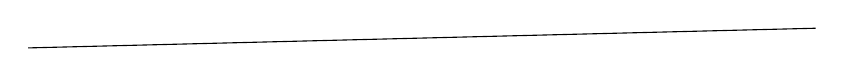
\begin{tikzpicture}\draw (0,0)--(10,0.25);\end{tikzpicture}}

\[
\mathbb H^i(\operatorname{Spec}\mathbf Z,\mathbf Z(1))=\begin{cases}0&\underset{\text{
\begin{tikzpicture}[baseline=0pt]\draw[line width=0.7pt] (0,0)--(0.28,0.08)--(0.04,-0.05)--(0.32,-0.14)--(0.28,0.03)--(0.12,-0.09)--(0.35,-0.18)--(0.26,0.02);\end{tikzpicture}}}{\text{si }}i\neq3\\\mathbf Z&\text{si }i=3\end{cases}
\]
\[
\mathbb H^i(\operatorname{Spec}\mathbf Z,\mathbf Z)=\begin{cases}0&\text{si }i\neq0\\\mathbf Z&\text{si }i=0\end{cases}
\]
\margin{$H^i(\operatorname{Spec}(\mathbf Z),\mathbf Q(n))\xrightarrow{\sim}H^i(U,\mathbf Q(n))$ si $U$ ouvert de Zariski de $\operatorname{Spec}\mathbf Z$ et $n\neq0$ (tout $i$).}

\margin{172}

\scanpage{174}

$\operatorname{Spec}\mathbf Z$

\figure{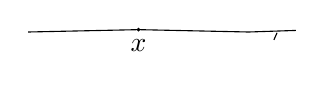
\begin{tikzpicture}\draw (0,0)--(1.4,0.03)--(2.8,0)--(3.4,0.02);\fill (1.4,0.03) circle (0.025);\node[below] at (1.4,0.03) {$x$};\draw (3.16,-0.01)--(3.12,-0.10);\end{tikzpicture}}

\[
i_x^!(M)=\unsure{P|R}i_x^*(M)(-1)[-2]
\]

\diagram{\begin{tikzcd}[column sep=small]
\cdots \arrow[r,no head]&H^{i-2}(x,i_x^*(M)(-1))\arrow[r]&H^i(X,M)\arrow[r,no head]&H^i(U,M)\arrow[r,no head]&H^{i-1}(x,i_x^*(M)(-1))\arrow[r]&\cdots
\end{tikzcd}}

\[
M=\underset{\sim}{\deleted{\mathbf Z}\inserted{\mathbf Q}}(n)
\]
\deleted{$H^i$}
\[
\left\{\begin{aligned}
&i\neq1,2,3\qquad H^i(X,M)\xrightarrow{\sim}H^i(U,M)\\[1em]
&0\longrightarrow H^1(X,M)\longrightarrow H^1(U,M)\longrightarrow H^0(S,i_x^*(M)(-1))\longrightarrow H^2(X,M)
\end{aligned}\right.
\]
\[
\begin{aligned}
&\hspace{3em}\longrightarrow H^2(U,M)\longrightarrow H^1(S,i_x^*(M)(-1))\longrightarrow H^3(X,M)\\[1em]
&\hspace{3em}\longrightarrow\underset{=\,0?}{H^3(U,M)}\longrightarrow0
\end{aligned}
\]
\margin{\figure{\begin{tikzpicture}[baseline=0pt]\draw (0,0)--(0,-1.2);\end{tikzpicture}} pas de miracle, car si $i\geq4$, les deux mbs doivent être $=0$.}

\[
M=\deleted{\mathbf Z_l}\mathbf Q_{\deleted{\unsure{l}}}(n),\qquad i_x^*(M)\unsure{(-1)|H_l}=\mathbf Q(n-1)_S
\]

\uline{Si $n\neq1$}\qquad $H^i(X,\mathbf Q(n))\xrightarrow{\sim}H^i(U,\mathbf Q(n))$\qquad\uline{tout $i$}
\margin{[est-ce nul ??]}

Si $n=1$
\diagram{\begin{tikzcd}[column sep=small]
0\arrow[r,no head]&H^1(X,\mathbf Q(1))\arrow[r]&H^1(U,\mathbf Q(1))\arrow[r]&\mathbf Q^S\arrow[r]&H^2(X,\mathbf Q(1))\arrow[r]&{}\\
{}&{}&H^2(U,\mathbf Q(1))\arrow[r]&\mathbf Q^S\arrow[r]&H^3(X,\mathbf Q(1))\arrow[r]&0
\end{tikzcd}}

$H^i(X,\mathbf Q(1))=0$ sauf pour $i=3$, où on \unsure{trouve} $\mathbf Q$ !

\margin{173}

\scanpage{176}

Lorsque \deleted{$X$ est} \deleted{\unsure{l'on est dans les conditions de}} les anneaux localisés stricts de $X$ sont factoriels, on tire aisément de (5.3.)
\[
H^1(X,\uline{\mathrm{Div}}_X)=0
\]
d'où \deleted{la proposition}

\uline{Proposition} 5.4. Supposons que l'on soit dans les conditions de 5.1. a), \inserted{$X$ étant irréductible de pt gén. $y$,} Alors les homomorphismes canoniques
\diagram{\begin{tikzcd}[column sep=large]
H^2(X,G_{mX})\arrow[r,no head]&H^2(X,R_X^*)\arrow[r]&H^2(y,G_{my})=\operatorname{Br}(y)
\end{tikzcd}}
sont injectifs.

Comme $\operatorname{Br}(X)\subset H^2(X,G_{mX})$, il s'ensuit

\uline{Corollaire} 5.5. Sous les $=^{s}$ conditions,
\diagram{\begin{tikzcd}[column sep=large]
\operatorname{Br}(X)\arrow[r,no head]&\operatorname{Br}(y)
\end{tikzcd}}
est injectif.

Ainsi, $\operatorname{Br}(X)$ s'identifie \inserted{alors} à un sous-groupe du groupe de Brauer $\operatorname{Br}(K)$ du corps des fonctions $K=k(y)$ de $X$.

\uline{Théorème} 5.6. \inserted{Soit $X$ un préschéma, $\xi\in H^2(X,G_m)$}
a) Si $X$ est un schéma local, et \deleted{$\xi\in H^2(X,G_{mX})$} pour que $\xi$ \deleted{provienne d'un élément de} \inserted{soit dans $\operatorname{Br}(X)$, il} f et s. qu'il existe un\deleted{e extension} morphisme fini étale surjectif (galoisien si on veut) $f:X'\longrightarrow X$, \deleted{tel que $\xi|X'\to0$} qui \deleted{splitte $\xi$} annule $\xi$.

\margin{175}

\scanpage{177}

\par\noindent
\deleted{\mbox{\begin{minipage}[c]{\linewidth}
\diagram{\begin{tikzcd}
\mu_n\arrow[r]&G_m\arrow[r,"n"]&G_m
\end{tikzcd}}
\end{minipage}}}
\par

$\mu$

\par\noindent
\deleted{\mbox{\begin{minipage}[c]{\linewidth}
\diagram{\begin{tikzcd}H^3(X,G_m)\arrow[r]&H^3\end{tikzcd}}
\end{minipage}}}
\par

\deleted{$H^i_x($}

\diagram{\begin{tikzcd}[column sep=small]
H^i_S(X,G_m)\arrow[r,no head]&H^i(X,G_m)\arrow[r]&H^i(U,G_m)\arrow[r,no head]&H^{\unsure{i+1|i-1}}_S(X,G_m)\arrow[r]&\underset{\text{\begin{tikzpicture}[x=1cm,y=1cm,baseline=0pt]\draw (0,0)--(.24,.01);\draw (.34,-.06)--(.43,-.08);\draw (.66,.02)--(.86,.02);\foreach \x/\y in {.15/-.16,.24/-.12,.40/-.19,.51/-.28,.73/-.14,.88/-.25,1.02/-.32,1.13/-.46,.87/-.56,1.05/-.63,.17/-.56,.18/-.68,.19/-.81,.21/-.94}{\fill (\x,\y) circle (.012);}\draw (.14,-.74)--(.20,-.75);\draw (.17,-.87)--(.24,-.89);\end{tikzpicture}}}{\unsure{\cdots}}
\end{tikzcd}}

\[
\uline{H}^i_x(G_m)=\begin{cases}
0&\text{si }i=0\\
\mathbf Z_x&\text{si }i=1\\
0&\text{si }i\geq2
\end{cases}
\]
\[
H^i_S(X,G_m)=H^{i-1}(S,\mathbf Z)=
\left\{\begin{array}{ll}
\unsure{0}&\text{si }i=0\\
\multicolumn{2}{l}{\left.\begin{array}{ll}
\mathbf Z^S&\text{si }i=1\\
0&\text{si }i=2\\
H^1(S,\mathbf Q/\mathbf Z)&\text{si }i=3
\end{array}\right]}\\
0&\text{si }i\geq4
\end{array}\right.
\]

\diagram{\begin{tikzcd}
0\arrow[r,no head]&\mathbf Z\arrow[r]&\mathbf Q\arrow[r,no head]&\mathbf Q/\mathbf Z\arrow[r,no head]&0
\end{tikzcd}}

\margin{$\begin{gathered}i=1,3\\i=0,2\end{gathered}$}
\figure{\begin{tikzpicture}\draw (0,0)--(0.6,1.2);\end{tikzpicture}}
Si $i\neq0,1,2,3$, $H^i(\bar X,G_m)\xrightarrow{\sim}H^i(U,G_m)$

\margin{pas de miracle, car les deux sont nuls.}

\diagram{\begin{tikzcd}[column sep=small,row sep=small]
0\arrow[r]&H^0(\bar X,G_m)\arrow[r]\arrow[d,equal]&H^0(\bar U,G_m)\arrow[r]&\mathbf Z^S\arrow[r]&H^1(\bar X,G_m)\arrow[r,no head]\arrow[d,equal]&H^1(\bar U,G_m)\arrow[r]\arrow[d,equal]&H^2_S(\bar X,G_m)\arrow[d,equal]\\
{}&\mathbf Z^*=\{+1,-1\}&{}&{}&0&0&0
\end{tikzcd}}

\diagram{\begin{tikzcd}[column sep=small,row sep=small]
0\arrow[r]&H^2(\bar X,G_m)\arrow[r]\arrow[d,equal]&H^2(\bar U,G_m)\arrow[r]&H^1(S,\mathbf Q/\mathbf Z)\arrow[r]\arrow[d,equal]&H^3(\bar X,G_m)\arrow[r]\arrow[d,equal]&H^3(\bar U,G_m)\arrow[r]\arrow[d,equal,"?" ]&0\\
{}&0&{}&(\mathbf Q/\mathbf Z)^S\arrow[r,phantom,"{\substack{\uline{\text{somme}}\\\uline{\text{des inv.}}}}"']&\mathbf Q/\mathbf Z&0&{}
\end{tikzcd}}

\margin{176}

\scanpage{179}
\par\noindent
\deleted{\mbox{\begin{minipage}[c]{\linewidth}
On peut supposer $X$ irréductible de pt générique $y$. L'inclusion $y-X$ définit une suite spectrale (pour la cohomologie étale)
\[
H^*(y,G_m)\Longleftarrow E_2^{pq}=H^p(X,\mathbb R^qi_*(G_m))
\]
Or \deleted{\unsure{comme les}} comme les $H^q(y,G_m)$ et les fibres de $R^qi_*(G_m)$, qui s'explicitent par de la cohomologie galoisienne, sont \deleted{des} groupes de torsion pour $q>0$, on trouve que \deleted{\unsure{l'on a} \unsure{dans|sur} les \unsure{les} groupes}
\[
(*)\qquad H^p(X,R_X^*)
\]
\deleted{, où $R_X=Ri_*(G_m)$}\inserted{est un groupe de torsion pour $p>0$,} où $R_X^*=\deleted{\unsure{Ri_*}}i_*(G_{m\,\unsure{x|y}})$ est le faisceau (étale) des fonctions rationnelles \inserted{non nulles} sur $X$. \deleted{(Ceci étant}
\end{minipage}}}
\par

D'autre part, \inserted{si $X$ est \inserted{noethérien} ``sans idéaux premiers immergés'',} on a la suite exacte
\[
(5.1.)\qquad 0-G_{mX}\longrightarrow R_X^*\longrightarrow\uline{\mathrm{Div}}_X\longrightarrow0
\]
où $\uline{\mathrm{Div}}_X$ est le faisceau \inserted{(pour la top\unsure{)}} (étale) des diviseurs (de Cartier) sur $X$, ce qui \deleted{montre que} \inserted{implique} compte tenu de $(*)$ que
\[
H^{i}(X,\uline{\mathrm{Div}}_X)\xrightarrow{\partial}H^{i+1}(X,\deleted{\unsure{R|D}}G_{mX})
\]
\margin{\uline{donner le} \uline{corollaire} 5.4.}
est bijectif mod torsion \deleted{\unsure{pour i|si}} si $i\geq1$. \deleted{Ainsi \unsure{on aura|ne sera pas} vraiment utilisé} L'hypothèse de factorialité d'autre part implique \deleted{l'isomorphisme} qu'on a un isomorphisme de faisceaux étales :
\margin{178}
